\newpage

\subsection{Contexto laboral}\subsubsection{Actividad y Ocupación}

En el Sistema de Jubilaciones y Pensiones administrado por el IPS, la
financiación se encuentra basada en los aportes obrero-patronales de los
asalariados, por lo que conocer el universo de potenciales afiliados es
de vital importancia.

Las estadísticas relacionadas al mercado de trabajo se obtienen de la
EPH. De acuerdo con estos datos, la población paraguaya total en el año
2020 es de 7.167.516 personas, de los cuales 5.094.469 tienen 15 o más
años de edad, que para los fines de este informe será considerada como
la población en edad de trabajar (PET), ésta representa un 71,1\% de la
población total. Una subpoblación de interés es la Población
Económicamente Activa (PEA) también llamada Fuerza de
Trabajo\footnote{Fuerza de trabajo, también conocida como Población Económicamente Activa (PEA) de acuerdo a la 19ª Conferencia Internacional de Estadístic
as del Trabajo - CIET.}, la cual está conformada por las personas
ocupadas y desocupadas. La Fuerza de Trabajo en Paraguay está compuesta
por un total de 3.678.114 de personas, que representan el 72,2\% de la
PET \footnote{Este resultado difiere de las 
publicaciones oficiales del INE por la definición especial considerada para la población en edad de trabajar.}.

La tasa de desocupación o desempleo abierto afectó en el año 2020 al
7,0\% de la PEA, lo que implica que alrededor de 256.678 personas
estaban sin trabajo y buscaron activamente empleo en el periodo de
referencia de la encuesta (últimos 7 días).

La estructura de la población con respecto a estos indicadores del
mercado laboral de las personas con 15 y más años de edad, para el
periodo 2013-2020, se presenta en la Tabla 2.

\begin{table}[H]
\begin{center}
\footnotesize
\caption{\bf{Estructura de la población. Periodo 2013-2020}}
\begin{tabular}{l|rrrrrr}
\begin{tabular}{llllllll}
\cline{1-8}
\multicolumn{1}{c}{} &
  \multicolumn{1}{|r}{PT} &
  \multicolumn{1}{r}{PET} &
  \multicolumn{1}{r}{PEA} &
  \multicolumn{1}{r}{PEI} &
  \multicolumn{1}{r}{PO} &
  \multicolumn{1}{r}{PD} &
  \multicolumn{1}{r}{NR} \\
\cline{1-8}
\multicolumn{1}{l}{Año} &
  \multicolumn{1}{|r}{} &
  \multicolumn{1}{r}{} &
  \multicolumn{1}{r}{} &
  \multicolumn{1}{r}{} &
  \multicolumn{1}{r}{} &
  \multicolumn{1}{r}{} &
  \multicolumn{1}{r}{} \\
\multicolumn{1}{l}{\hspace{1em}2013} &
  \multicolumn{1}{|r}{6.485.377} &
  \multicolumn{1}{r}{4.422.659} &
  \multicolumn{1}{r}{3.156.825} &
  \multicolumn{1}{r}{1.265.630} &
  \multicolumn{1}{r}{2.997.615} &
  \multicolumn{1}{r}{159.210} &
  \multicolumn{1}{r}{204} \\
\multicolumn{1}{l}{\hspace{1em}2014} &
  \multicolumn{1}{|r}{6.581.971} &
  \multicolumn{1}{r}{4.535.155} &
  \multicolumn{1}{r}{3.166.411} &
  \multicolumn{1}{r}{1.368.744} &
  \multicolumn{1}{r}{2.976.862} &
  \multicolumn{1}{r}{189.549} &
  \multicolumn{1}{r}{0} \\
\multicolumn{1}{l}{\hspace{1em}2015} &
  \multicolumn{1}{|r}{6.678.731} &
  \multicolumn{1}{r}{4.657.248} &
  \multicolumn{1}{r}{3.233.111} &
  \multicolumn{1}{r}{1.424.137} &
  \multicolumn{1}{r}{3.061.380} &
  \multicolumn{1}{r}{171.731} &
  \multicolumn{1}{r}{0} \\
\multicolumn{1}{l}{\hspace{1em}2016} &
  \multicolumn{1}{|r}{6.775.786} &
  \multicolumn{1}{r}{4.710.766} &
  \multicolumn{1}{r}{3.322.812} &
  \multicolumn{1}{r}{1.387.177} &
  \multicolumn{1}{r}{3.122.747} &
  \multicolumn{1}{r}{200.065} &
  \multicolumn{1}{r}{777} \\
\multicolumn{1}{l}{\hspace{1em}2017} &
  \multicolumn{1}{|r}{6.873.496} &
  \multicolumn{1}{r}{4.821.570} &
  \multicolumn{1}{r}{3.406.276} &
  \multicolumn{1}{r}{1.415.294} &
  \multicolumn{1}{r}{3.228.636} &
  \multicolumn{1}{r}{177.640} &
  \multicolumn{1}{r}{0} \\
\multicolumn{1}{l}{\hspace{1em}2018} &
  \multicolumn{1}{|r}{6.971.229} &
  \multicolumn{1}{r}{4.897.047} &
  \multicolumn{1}{r}{3.517.575} &
  \multicolumn{1}{r}{1.379.472} &
  \multicolumn{1}{r}{3.317.775} &
  \multicolumn{1}{r}{199.800} &
  \multicolumn{1}{r}{0} \\
\multicolumn{1}{l}{\hspace{1em}2019} &
  \multicolumn{1}{|r}{7.069.327} &
  \multicolumn{1}{r}{4.988.971} &
  \multicolumn{1}{r}{3.626.368} &
  \multicolumn{1}{r}{1.362.603} &
  \multicolumn{1}{r}{3.422.331} &
  \multicolumn{1}{r}{204.037} &
  \multicolumn{1}{r}{0} \\
\multicolumn{1}{l}{\hspace{1em}2020} &
  \multicolumn{1}{|r}{7.167.516} &
  \multicolumn{1}{r}{5.094.469} &
  \multicolumn{1}{r}{3.678.114} &
  \multicolumn{1}{r}{1.416.355} &
  \multicolumn{1}{r}{3.421.436} &
  \multicolumn{1}{r}{256.678} &
  \multicolumn{1}{r}{0} \\
\cline{1-8}
\end{tabular}

\end{tabular}
                    \item \footnotesize Fuente : Encuesta Permanente de Hogares. 
                    \item \footnotesize Nota : PT (Población Total), PET (Población en Edad de Trabajar) PEA (Población Económicamente Activa), PEI (Población Económicamente Inactiva), PO (Población Ocupada), PD (Población Desocupada) NR (No Responde). 
\end{center}
\end{table}

\begin{center}
\end{center}\begin{figure}[!ht]
                    \caption{Estructura del mercado de trabajo. Año 2020}
  \centering
  \hspace*{-80pt}
  \begin{tikzpicture}[node distance = 1cm, auto]
  
          % Place nodes
    \node [block] (p) { \textbf{Población Total} 7.167.516 (100\%)};
    \node [block,  below left=1cm and -0.3cm of p](pet) {\textbf{Población en Edad de Trabajar  (mayor a 14 años)} 5.094.469 (71.07\%)};
    \node [block,  below right=1cm and -0.3cm of p](pm15) {\textbf{Población menor a 15 años} 2.073.047. (28.92\%)};
    \node [block,  below left=1cm and -0.3cm of pet](pea) {\textbf{Población Económicamente Activa (PEA)} 3.678.114 (72.84\%)};
    \node [block,  below right=1cm and -0.3cm of pet](pei) {\textbf{{Población Económicamente} Inactiva} 1.416.355. (28.04\%)};
         \node [block,  below left=1cm and -0.3cm of pea](o) {\textbf{Ocupados} 3.421.436 (93.02\%)};
    \node [block,  below right=1cm and -0.3cm of pea](d) {\textbf{Desocupados} 256.678 (6.97\%)}; 
    % edges
         \path [line] (p) -- (pet);
         \path [line] (p) -- (pm15);
         \path [line] (pet) -- (pea);
         \path [line] (pet) -- (pei);
         \path [line] (pea) -- (o);
         \path [line] (pea) -- (d);
  \end{tikzpicture}
\end{figure}

La Tasa de Actividad se define como el cociente entre la Población
Económicamente Activa y la Población en Edad de Trabajar de 15 y más
años de edad, en tanto que la Tasa de Ocupación se calcula como el
cociente entre la Población Ocupada y la Población Económicamente
Activa.

Al observar la evolución de dichas tasas para el periodo 2013-2020, no
se presentan variaciones significativas entre los años 2013 y 2019. En
tanto que, para el año 2020 se aprecia una leve disminución de la tasa
de ocupación en 1,35 puntos porcentuales , pasando de 94,37\% en el año
2019 a 93,02\% para el año 2020.

\begin{figure}[H]
\begin{center}
                    \caption{Tasas de Actividad y Ocupación. Periodo 2013-2020}
                    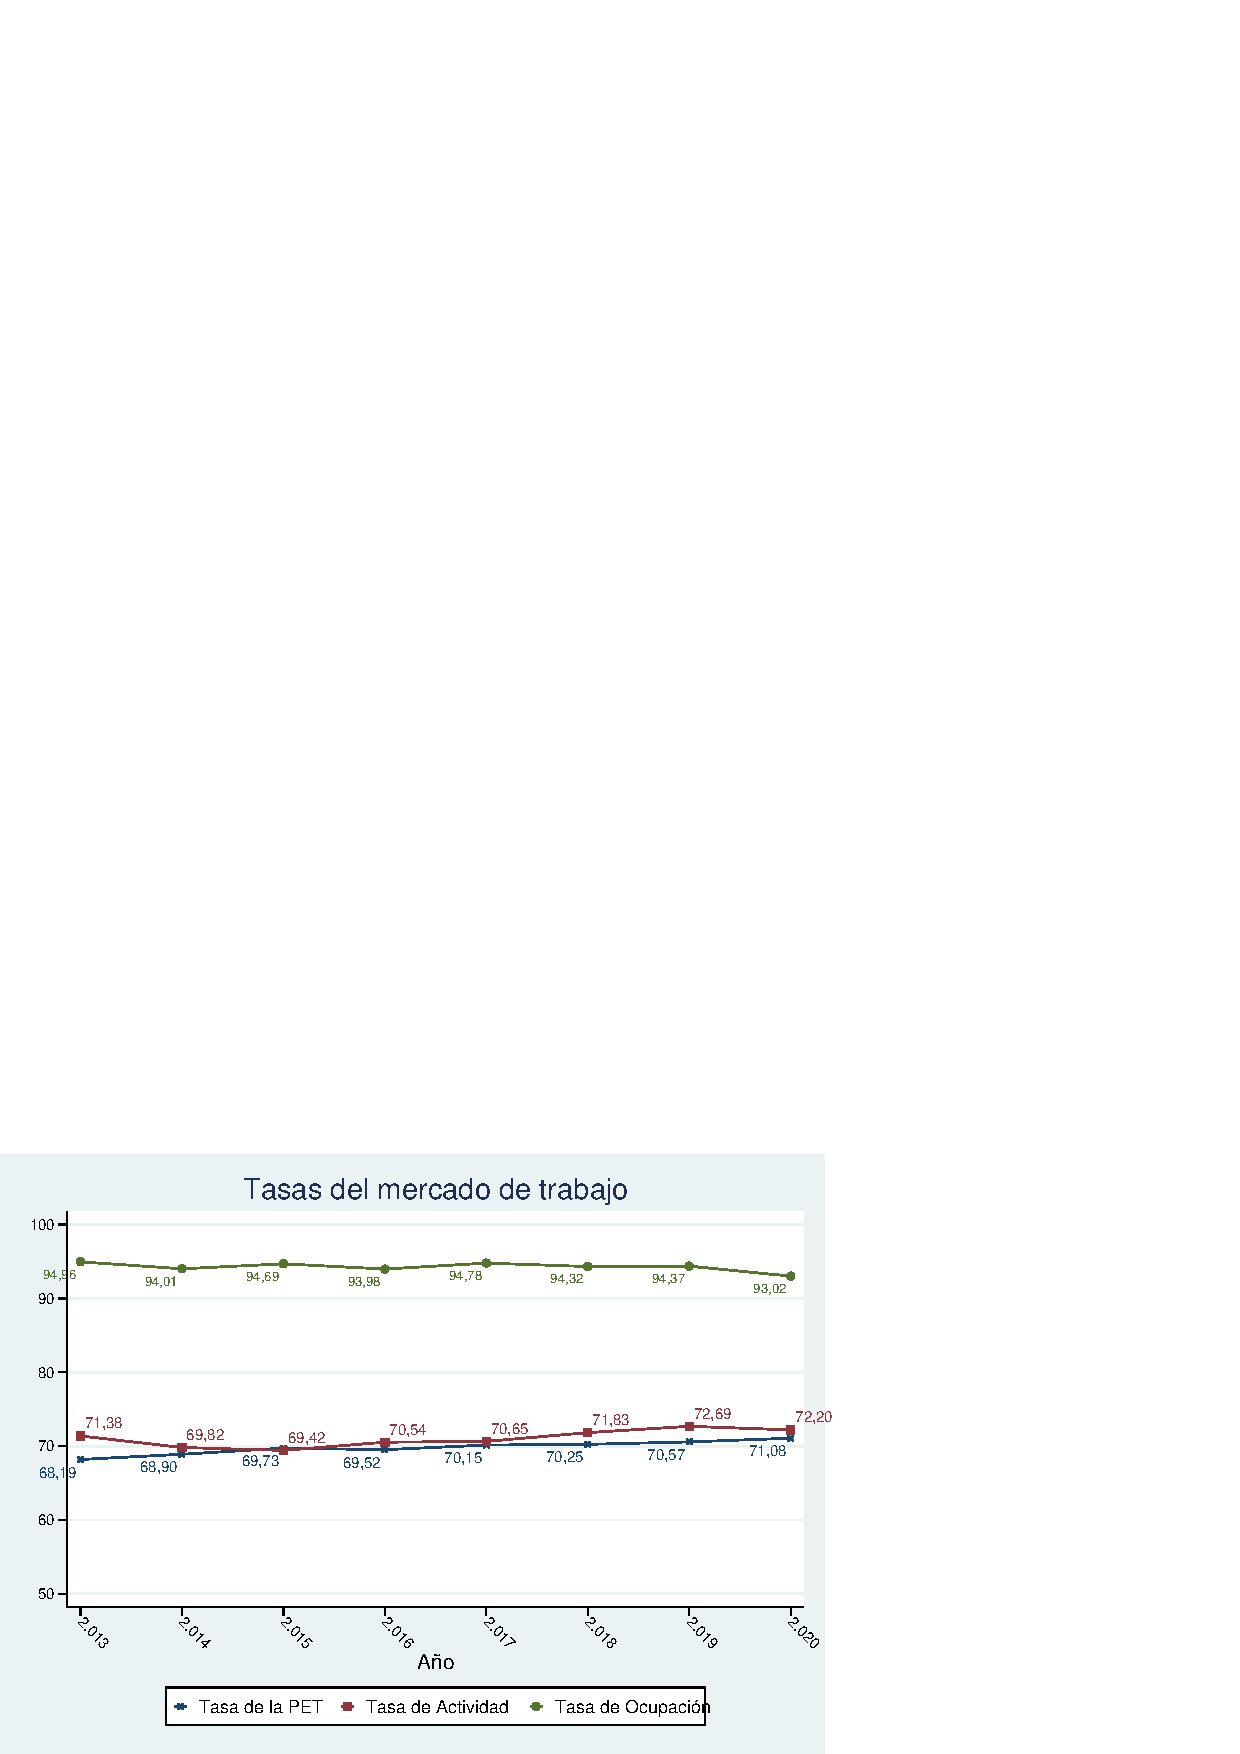
\includegraphics[scale=0.55]{EPH_tasas_peaa.png}
                                    \item \footnotesize Fuente : Instituto Nacional de Estadística.
                                    \item \footnotesize Nota : Tasa de la Población en Edad de Trabajar=PET/PT, Tasa de Actividad=PEA/PET, Tasa de Ocupación=PO/PEA
                    \end{center}
\end{figure}

La participación de la mujer paraguaya en el mercado laboral ha
aumentado en la última década. En la Figura 12 se observa el
comportamiento de la tasa de ocupación por sexo y por tramos de edad.

\begin{figure}[H]
\begin{center}
                    \caption{Evolución de la Tasa de Actividad y de Ocupación por año, según sexo}
                    \includegraphics[scale=0.55]{EPH_tasas_sexo_ocup_act.png}
                                    \item \footnotesize Fuente : Instituto Nacional de Estadística.
                                    \item \footnotesize Nota : Tasa de Ocupación=PO/PEA
                    \end{center}
\end{figure}

\begin{figure}[H]
\begin{center}
                    \caption{Tasas de Actividad y de Ocupación por tramos de edad, según sexo (Año 2020)}
                    \includegraphics[scale=0.55]{EPH_tasasgq_ocupacion_actividad.png}
                                    \item \footnotesize Fuente : Instituto Nacional de Estadística.
                                    \item \footnotesize Nota : Tasa de Ocupación=PO/PEA
                    \end{center}
\end{figure}

La Tasa de Actividad para el año 2020 desagregada por sexo, muestra que
del total de hombres en edad de trabajar un 84,5\% participa en el
mercado laboral, mientras que del total de mujeres en edad de trabajar
un 60,4\% participa en el mercado laboral.

En la distribución de la tasa por sexo según tramos de edad, las curvas
presentan el siguiente comportamiento: valores bajos para los tramos en
los cuales las personas asisten a la escuela/universidad, valores altos
para edades intermedias y baja partic ipación en las edades de retiro y
vejez.

Cabe destacar que, la Tasa de Actividad de las mujeres es inferior a la
de los hombres en todos los tramos etarios observados. En el caso de los
hombres, éstos poseen prácticamente una participación total (cercana al
100\%) en los grupos de edad compren didos entre los 30 - 49 años.

\subsubsection{Asalarización}

Cuando se analiza la Población Activa Ocupada, la segmentación de los
trabajadores según tipo de ocupación indica que el 37,6\% de los mismos
corresponden a mano de obra independiente (cuenta propia y empleador o
patrón). El 54,6\% se encuentra en rela ción de dependencia
clasificándose en Privado 37,9\%, Público 9,9\% y Doméstico 6,9\%. Y el
restante 7,8\% pertenece a la categoría de trabajadores familiares no
remunerados.

La importancia de conocer la relación laboral del trabajador,
\textit{"dependiente / independiente"} o \textit{"publico / privado"},
radica en que, el ámbito de obligatoriedad para aportar al Sistema de
Jubilaciones y Pensiones del IPS se restringe al\\
textit\{``Empleado / Obrero Privado''\} y al
\textit{"Empleado Doméstico \footnote{Clasificación de Categoría Ocupacional utilizada por la EPH del INE, corresponde al tipo de relación de dependencia en el trabajo con la entidad empleadora. Se distinguen den
tro de este tipo de relación: al patrón o socio activo, trabajador por cuenta propia, empleado u obrero público, empleado u obrero de empresa privada, servicio doméstico (asalariado) y trabajador familiar no remunerado.}"}.

\begin{table}[H]
\begin{center}
\scriptsize
\caption{\bf{Población por categoría de ocupación}}
\begin{tabular}{l|rrrrrr}
\begin{tabular}{lllllllll}
\cline{1-9}
\multicolumn{1}{c}{} &
  \multicolumn{8}{|c}{Año} \\
\multicolumn{1}{c}{} &
  \multicolumn{1}{|r}{2013} &
  \multicolumn{1}{r}{2014} &
  \multicolumn{1}{r}{2015} &
  \multicolumn{1}{r}{2016} &
  \multicolumn{1}{r}{2017} &
  \multicolumn{1}{r}{2018} &
  \multicolumn{1}{r}{2019} &
  \multicolumn{1}{r}{2020} \\
\cline{1-9}
\multicolumn{1}{l}{Categoría de Ocupación} &
  \multicolumn{1}{|r}{} &
  \multicolumn{1}{r}{} &
  \multicolumn{1}{r}{} &
  \multicolumn{1}{r}{} &
  \multicolumn{1}{r}{} &
  \multicolumn{1}{r}{} &
  \multicolumn{1}{r}{} &
  \multicolumn{1}{r}{} \\
\multicolumn{1}{l}{\hspace{1em}Empleado / obrero público} &
  \multicolumn{1}{|r}{334.482} &
  \multicolumn{1}{r}{303.628} &
  \multicolumn{1}{r}{348.234} &
  \multicolumn{1}{r}{314.055} &
  \multicolumn{1}{r}{295.901} &
  \multicolumn{1}{r}{340.031} &
  \multicolumn{1}{r}{347.965} &
  \multicolumn{1}{r}{337.401} \\
\multicolumn{1}{l}{\hspace{1em}Empleado / obrero privado} &
  \multicolumn{1}{|r}{1.111.782} &
  \multicolumn{1}{r}{1.183.150} &
  \multicolumn{1}{r}{1.173.650} &
  \multicolumn{1}{r}{1.214.963} &
  \multicolumn{1}{r}{1.275.933} &
  \multicolumn{1}{r}{1.297.794} &
  \multicolumn{1}{r}{1.337.879} &
  \multicolumn{1}{r}{1.295.107} \\
\multicolumn{1}{l}{\hspace{1em}Empleador o patrón} &
  \multicolumn{1}{|r}{193.498} &
  \multicolumn{1}{r}{194.529} &
  \multicolumn{1}{r}{147.142} &
  \multicolumn{1}{r}{159.379} &
  \multicolumn{1}{r}{172.382} &
  \multicolumn{1}{r}{178.991} &
  \multicolumn{1}{r}{181.801} &
  \multicolumn{1}{r}{162.522} \\
\multicolumn{1}{l}{\hspace{1em}Trabajador por cuenta propia} &
  \multicolumn{1}{|r}{934.893} &
  \multicolumn{1}{r}{923.492} &
  \multicolumn{1}{r}{930.815} &
  \multicolumn{1}{r}{985.764} &
  \multicolumn{1}{r}{1.004.297} &
  \multicolumn{1}{r}{1.006.739} &
  \multicolumn{1}{r}{1.047.378} &
  \multicolumn{1}{r}{1.122.778} \\
\multicolumn{1}{l}{\hspace{1em}Trabajador familiar no remunerado} &
  \multicolumn{1}{|r}{199.911} &
  \multicolumn{1}{r}{164.320} &
  \multicolumn{1}{r}{248.157} &
  \multicolumn{1}{r}{235.602} &
  \multicolumn{1}{r}{240.814} &
  \multicolumn{1}{r}{243.886} &
  \multicolumn{1}{r}{245.759} &
  \multicolumn{1}{r}{268.295} \\
\multicolumn{1}{l}{\hspace{1em}Empleado doméstico} &
  \multicolumn{1}{|r}{220.529} &
  \multicolumn{1}{r}{207.382} &
  \multicolumn{1}{r}{213.300} &
  \multicolumn{1}{r}{211.684} &
  \multicolumn{1}{r}{237.093} &
  \multicolumn{1}{r}{249.868} &
  \multicolumn{1}{r}{259.633} &
  \multicolumn{1}{r}{235.333} \\
\multicolumn{1}{l}{\hspace{1em}NR} &
  \multicolumn{1}{|r}{2.520} &
  \multicolumn{1}{r}{361} &
  \multicolumn{1}{r}{82} &
  \multicolumn{1}{r}{1.300} &
  \multicolumn{1}{r}{2.216} &
  \multicolumn{1}{r}{466} &
  \multicolumn{1}{r}{1.916} &
  \multicolumn{1}{r}{} \\
\multicolumn{1}{l}{\hspace{1em}Total} &
  \multicolumn{1}{|r}{2.997.615} &
  \multicolumn{1}{r}{2.976.862} &
  \multicolumn{1}{r}{3.061.380} &
  \multicolumn{1}{r}{3.122.747} &
  \multicolumn{1}{r}{3.228.636} &
  \multicolumn{1}{r}{3.317.775} &
  \multicolumn{1}{r}{3.422.331} &
  \multicolumn{1}{r}{3.421.436} \\
\cline{1-9}
\end{tabular}

\end{tabular}
                    \item \footnotesize Fuente : Encuesta Permanente de Hogares. 
                    \item \footnotesize Nota : Trabajadores ocupados mayores de 14 años.
\end{center}
\end{table}

\begin{table}[H]
\begin{center}
\scriptsize
\caption{\bf{Población por categoría de ocupación (en porcentaje). Periodo 2013-2020}}
\begin{tabular}{l|rrrrrr}
\begin{tabular}{lllllllll}
\cline{1-9}
\multicolumn{1}{c}{} &
  \multicolumn{8}{|c}{Año} \\
\multicolumn{1}{c}{} &
  \multicolumn{1}{|r}{2013} &
  \multicolumn{1}{r}{2014} &
  \multicolumn{1}{r}{2015} &
  \multicolumn{1}{r}{2016} &
  \multicolumn{1}{r}{2017} &
  \multicolumn{1}{r}{2018} &
  \multicolumn{1}{r}{2019} &
  \multicolumn{1}{r}{2020} \\
\cline{1-9}
\multicolumn{1}{l}{Categoría de Ocupación} &
  \multicolumn{1}{|r}{} &
  \multicolumn{1}{r}{} &
  \multicolumn{1}{r}{} &
  \multicolumn{1}{r}{} &
  \multicolumn{1}{r}{} &
  \multicolumn{1}{r}{} &
  \multicolumn{1}{r}{} &
  \multicolumn{1}{r}{} \\
\multicolumn{1}{l}{\hspace{1em}Empleado / obrero público} &
  \multicolumn{1}{|r}{11,16} &
  \multicolumn{1}{r}{10,20} &
  \multicolumn{1}{r}{11,38} &
  \multicolumn{1}{r}{10,06} &
  \multicolumn{1}{r}{9,16} &
  \multicolumn{1}{r}{10,25} &
  \multicolumn{1}{r}{10,17} &
  \multicolumn{1}{r}{9,86} \\
\multicolumn{1}{l}{\hspace{1em}Empleado / obrero privado} &
  \multicolumn{1}{|r}{37,09} &
  \multicolumn{1}{r}{39,74} &
  \multicolumn{1}{r}{38,34} &
  \multicolumn{1}{r}{38,91} &
  \multicolumn{1}{r}{39,52} &
  \multicolumn{1}{r}{39,12} &
  \multicolumn{1}{r}{39,09} &
  \multicolumn{1}{r}{37,85} \\
\multicolumn{1}{l}{\hspace{1em}Empleador o patrón} &
  \multicolumn{1}{|r}{6,46} &
  \multicolumn{1}{r}{6,53} &
  \multicolumn{1}{r}{4,81} &
  \multicolumn{1}{r}{5,10} &
  \multicolumn{1}{r}{5,34} &
  \multicolumn{1}{r}{5,39} &
  \multicolumn{1}{r}{5,31} &
  \multicolumn{1}{r}{4,75} \\
\multicolumn{1}{l}{\hspace{1em}Trabajador por cuenta propia} &
  \multicolumn{1}{|r}{31,19} &
  \multicolumn{1}{r}{31,02} &
  \multicolumn{1}{r}{30,41} &
  \multicolumn{1}{r}{31,57} &
  \multicolumn{1}{r}{31,11} &
  \multicolumn{1}{r}{30,34} &
  \multicolumn{1}{r}{30,60} &
  \multicolumn{1}{r}{32,82} \\
\multicolumn{1}{l}{\hspace{1em}Trabajador familiar no remunerado} &
  \multicolumn{1}{|r}{6,67} &
  \multicolumn{1}{r}{5,52} &
  \multicolumn{1}{r}{8,11} &
  \multicolumn{1}{r}{7,54} &
  \multicolumn{1}{r}{7,46} &
  \multicolumn{1}{r}{7,35} &
  \multicolumn{1}{r}{7,18} &
  \multicolumn{1}{r}{7,84} \\
\multicolumn{1}{l}{\hspace{1em}Empleado doméstico} &
  \multicolumn{1}{|r}{7,36} &
  \multicolumn{1}{r}{6,97} &
  \multicolumn{1}{r}{6,97} &
  \multicolumn{1}{r}{6,78} &
  \multicolumn{1}{r}{7,34} &
  \multicolumn{1}{r}{7,53} &
  \multicolumn{1}{r}{7,59} &
  \multicolumn{1}{r}{6,88} \\
\multicolumn{1}{l}{\hspace{1em}NR} &
  \multicolumn{1}{|r}{0,08} &
  \multicolumn{1}{r}{0,01} &
  \multicolumn{1}{r}{0,00} &
  \multicolumn{1}{r}{0,04} &
  \multicolumn{1}{r}{0,07} &
  \multicolumn{1}{r}{0,01} &
  \multicolumn{1}{r}{0,06} &
  \multicolumn{1}{r}{} \\
\multicolumn{1}{l}{\hspace{1em}Total} &
  \multicolumn{1}{|r}{100,00} &
  \multicolumn{1}{r}{100,00} &
  \multicolumn{1}{r}{100,00} &
  \multicolumn{1}{r}{100,00} &
  \multicolumn{1}{r}{100,00} &
  \multicolumn{1}{r}{100,00} &
  \multicolumn{1}{r}{100,00} &
  \multicolumn{1}{r}{100,00} \\
\cline{1-9}
\end{tabular}

\end{tabular}
                    \item \footnotesize Fuente : Encuesta Permanente de Hogares. 
                    \item \footnotesize Nota : Trabajadores ocupados mayores de 14 años.
\end{center}
\end{table}

En cuanto a las tendencias, se puede ver que la distribución de los
porcentajes de trabajadores por tipo de ocupación es similar en los
últimos 8 años.

El sector privado ha tenido un aumento sostenido entre los años 2013 y
2019, pasando de un valor aproximado de 37,1\% a un valor de 39,1\%.
Para el año 2020 esta proporción disminuyó levemente alcanzando un valor
de 37,9\%.

Por otra parte, el sector de los empleados por cuenta propia ha tenido
un aumento, pasando de un valor de 31,2\% en el año 2013 a un valor de
32,8\% para el año 2020. Las demás categorías no han presentado
variaciones importantes.

\begin{figure}[H]
\begin{center}
                    \caption{Evolución de la cantidad de trabajadores por categoría de ocupación. Periodo 2013-2020}
                    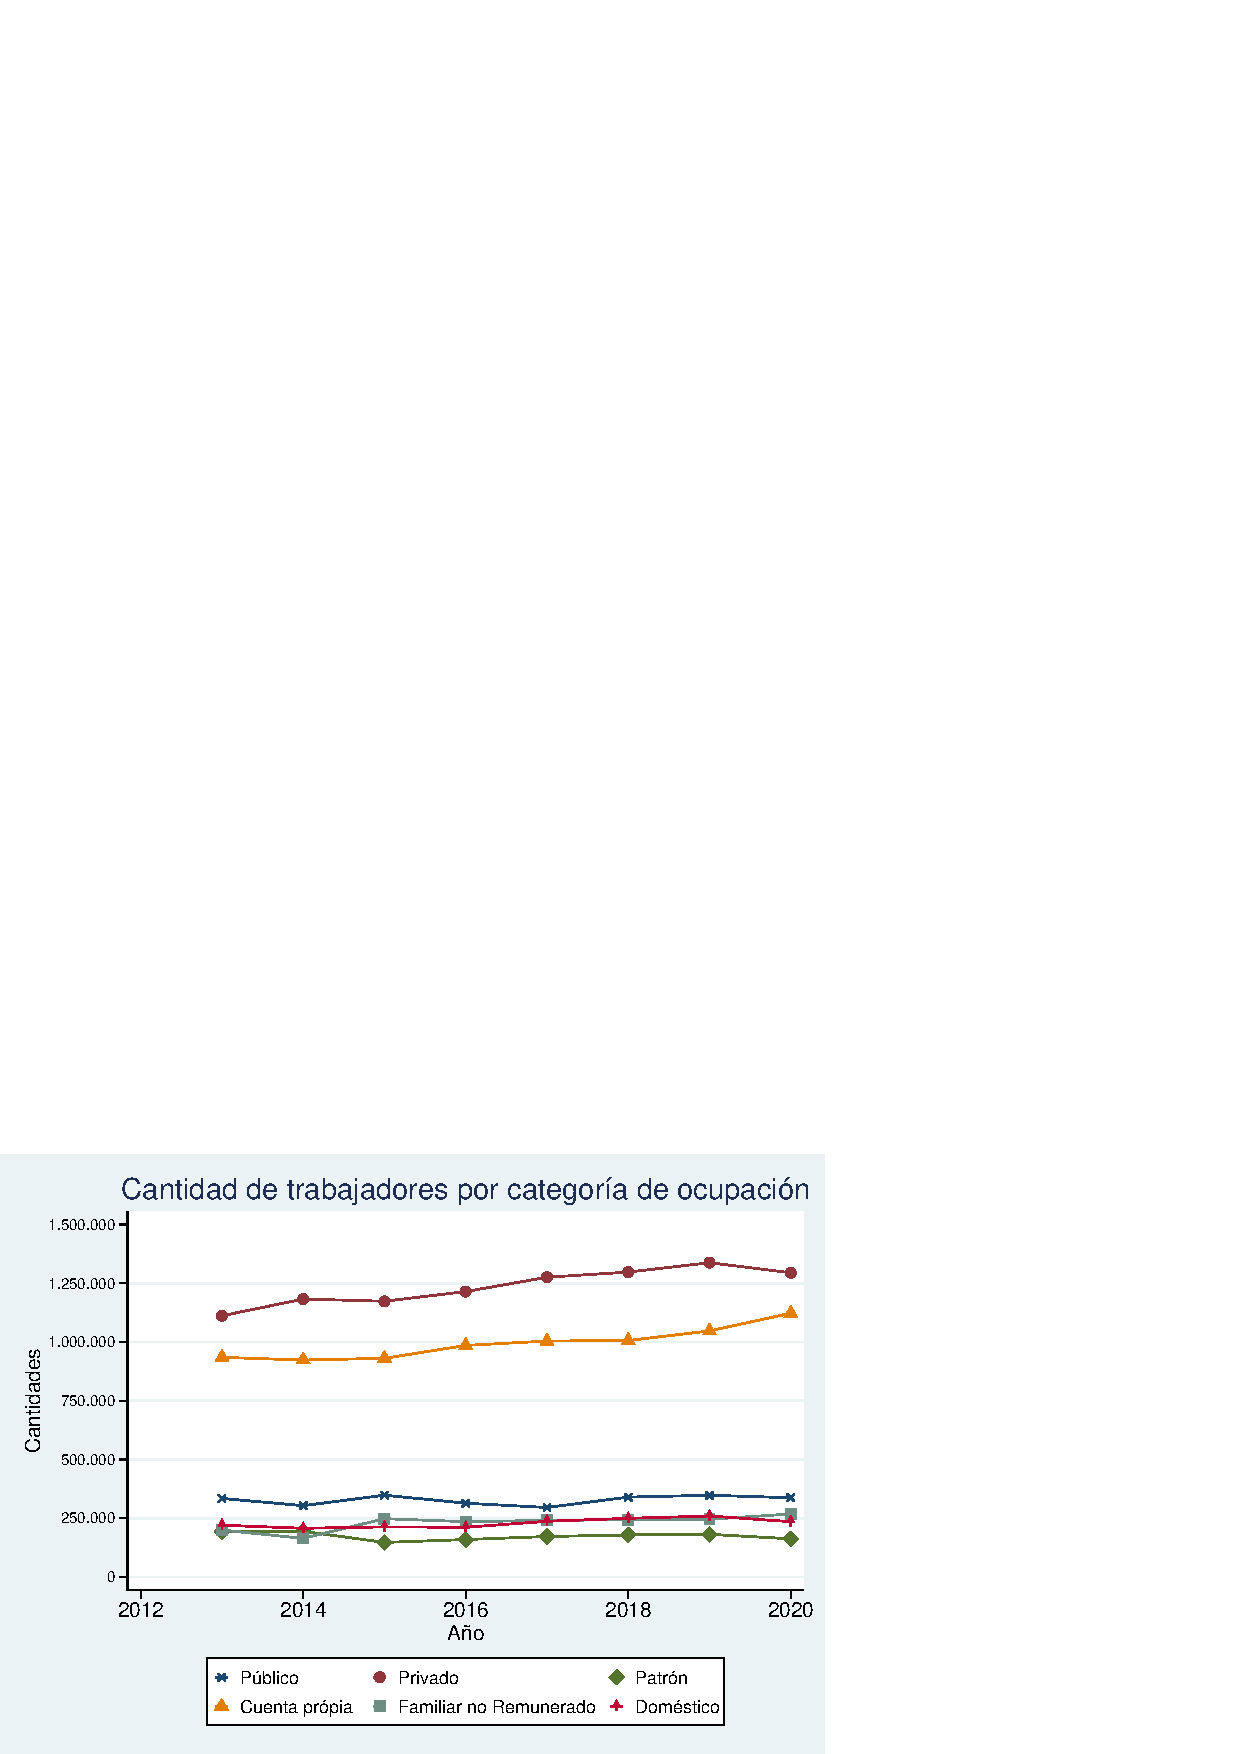
\includegraphics[scale=0.55]{EPH_catepea.png}
                                    \item \footnotesize Fuente : Encuesta Permanente de Hogares.
                                    %\item \footnotesize Nota : 
                    \end{center}
\end{figure}
